\chapter{\IfLanguageName{dutch}{Opstellen Dashboard}{Opstellen Dashboard}}%
\label{ch:Opstellen Dashboard}

\section{Kibana}

Het heeft veel langer geduurd dan verwacht om de ELK-integratie op te zetten. Het ELK-team had niet genoeg tijd vanwege ander werk dat ze moesten verrichten. Dit betekent dat er voor het onderzoek niet genoeg tijd zal zijn om het dashboard tijdig op te zetten en te analyseren. Op het moment van schrijven zijn nog steeds de juiste machtigingen gegeven om dashboards aan te maken. Het onderzoek zal nu doorgaan met wat we hebben en zal theoretisch concluderen of een dashboard de moeite waard is voor MFPOSS. Dit neemt een groot stuk uit het onderzoek maar geeft ons nog wel genoeg om tot een conclusie te komen.

\subsection{Toegang tot Kibana}
De huidige situatie is dat er toegang is verleend aan de testomgeving voor Kibana, via een link die door het ELK-team is verstrekt. Hier kan worden gezocht naar "Mainframe systemlogs" om enkele van onze logs te bekijken die handmatig zijn geüpload. Er waren enkele problemen met toegangsrechten en permissies met onze gebruikelijke accounts. Om dit probleem op te lossen, heeft het ELK-team een account gemaakt dat aan de juiste voorwaarden voldoet. Met deze gegevens kunnen we al een aantal zaken testen die op het dashboard kunnen verschijnen.

\subsection{Kibana Discover}
In dit hoofdstuk gaan we onderzoeken of we met de testlogs kunnen zien of het theoretisch mogelijk is om een dashboard te maken dat geschikt is voor MFPOSS. Dit doen we door de gegevens apart te visualiseren en de panelen van de mockup na te bootsen.

\subsubsection{Probleem twee}
Naast het eerder besproken probleem met de permissies was er ook een probleem met de logs die we hadden geüpload. De volledige logboekmelding, inclusief datum, tijd, cnslname en terminal, bevond zich in hetzelfde veld, terwijl alle andere velden leeg waren. Dit probleem kon worden opgelost door de logs handmatig opnieuw te uploaden. De onjuiste gegevens staan nog steeds in ELK, maar kunnen eenvoudig worden vermeden. Daarnaast zijn de datum- en tijdvelden niet zoals verwacht, maar gelukkig kunnen we er nog steeds mee werken. Deze moeten later worden aangepast door een lid van het ELK-team.

\subsubsection{Paneel één}
Het eerste paneel op de mockup had tot doel een weergave te geven van het aantal keren dat elk type terminal in de laatste 7 dagen voorkwam. Voor dit specifieke paneel was er niet genoeg gegevens beschikbaar over meerdere dagen. Daarom hebben we ervoor gekozen om het aantal keren dat een terminal voorkwam in een kolomgrafiek weer te geven. Dit had ook een lijngrafiek kunnen zijn met het aantal records in de laatste zeven dagen. Dit paneel wordt als succesvol beschouwd.

\begin{figure}[h]
    \centering
    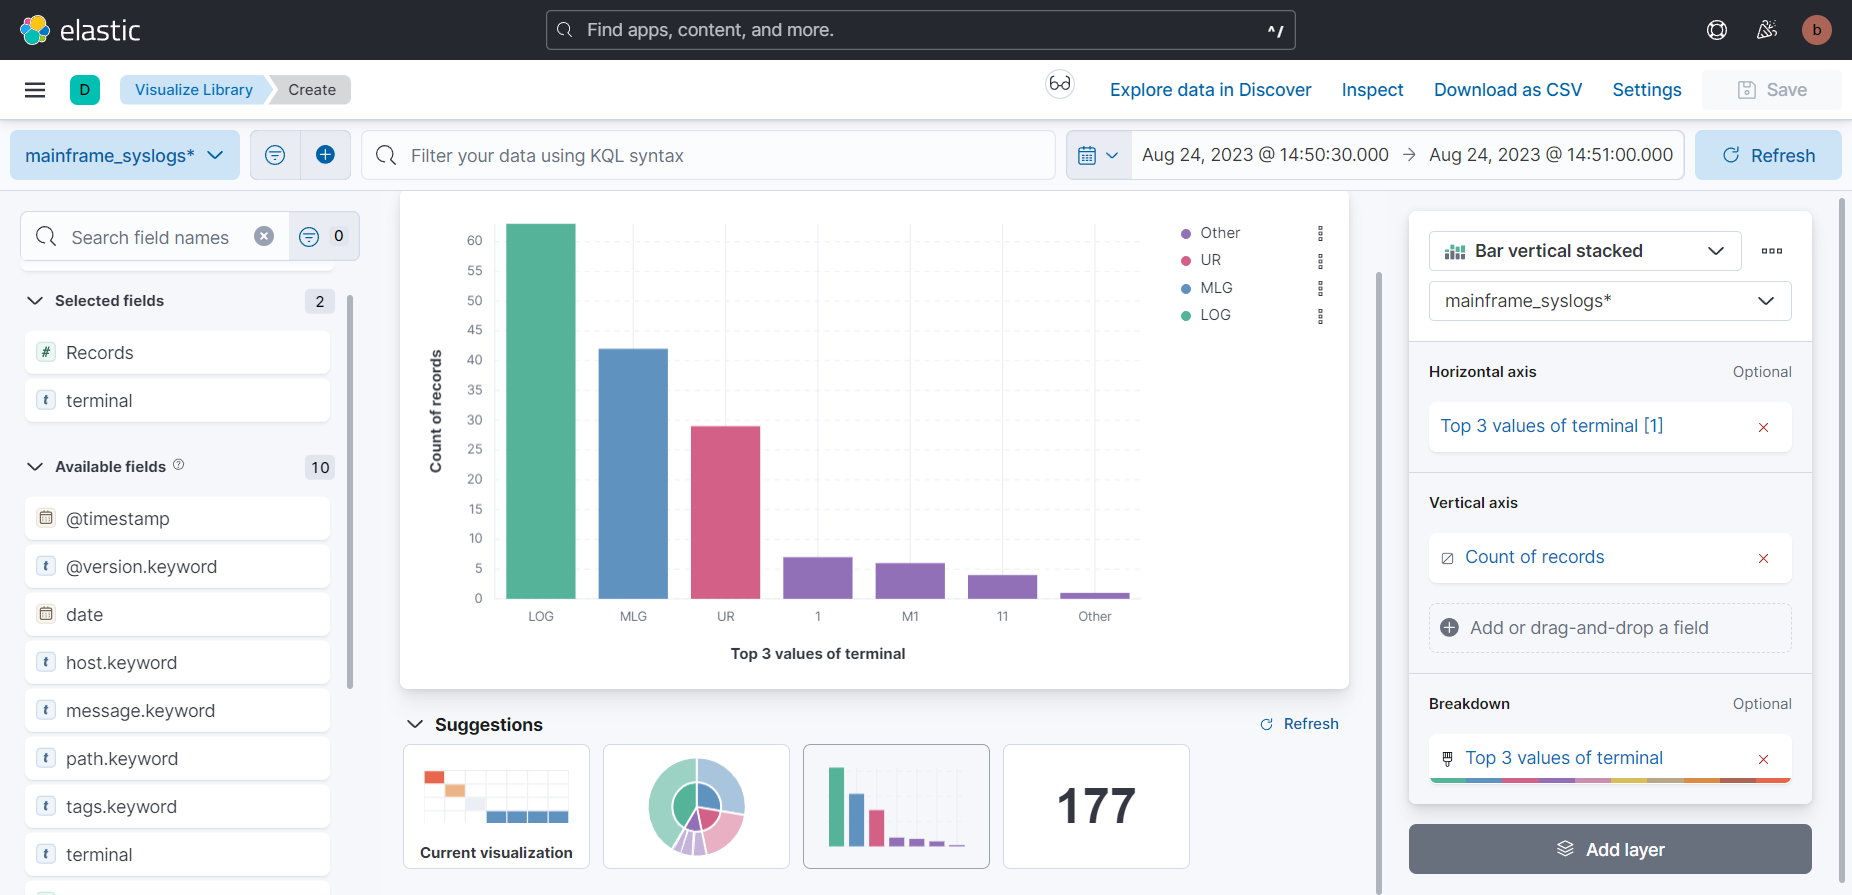
\includegraphics[width=0.50\linewidth]{bachproef//graphics/kibana_bar_chart.png}
    \caption{Een kolomgrafiek van het aantal keren dat een terminal voorkwam}
    \label{fig:Een kolomgrafiek van het aantal keren dat een terminal voorkwam}
\end{figure}

\subsubsection{Paneel twee}
Paneel twee van de mockup was een optelling van alle rijen in het meest recente log. Dit is succesvol gerepliceerd in Kibana. Het kan worden gezien in figuur 5.2. Er zijn ook andere interessante statistieken die MFPOSS mogelijk kan gebruiken.

\begin{figure}[h]
    \centering
    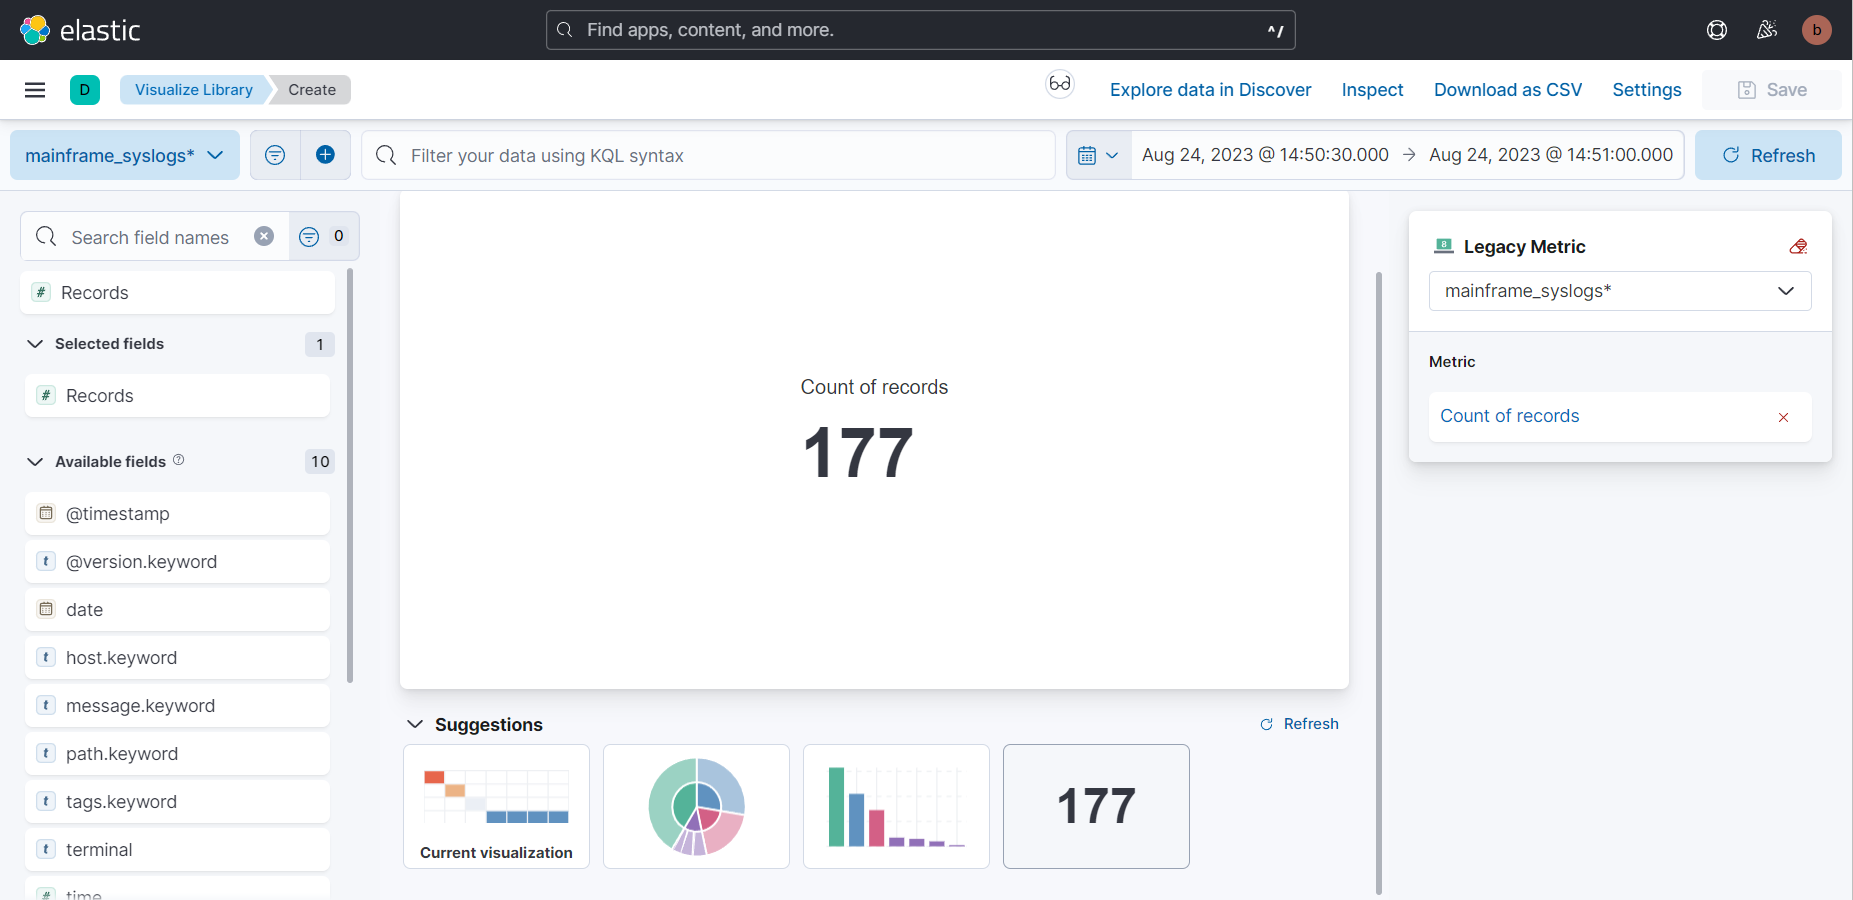
\includegraphics[width=0.50\linewidth]{bachproef//graphics/kibana_record_panel.png}
    \caption{De replicatie van paneel twee}
    \label{fig:De replicatie van paneel twee}
\end{figure}

\subsubsection{Paneel drie}
Paneel drie zou normaal gesproken deviatiedetectie bevatten, maar aangezien dit niet wordt gebruikt in Colruyt, is besloten om van paneel drie een weergave te maken van het meest voorkomende logbericht. Dit kan met minimale extra inspanning worden gedaan. Aangezien het enigszins vergelijkbaar is met paneel één, bespreken we hier ook kort de mogelijkheden om snel statistieken te bekijken. Dit kan worden gedaan door te hoveren over een veld of door de veldstatistieken tab te gebruiken. Een ervaren MFPOSS-medewerker zou hier in principe de mogelijkheid hebben om te beoordelen of er een probleem of afwijking is. De volgende afbeeldingen laten zien hoe deze statistieken eruit zien.

\begin{figure}[h]
    \centering
    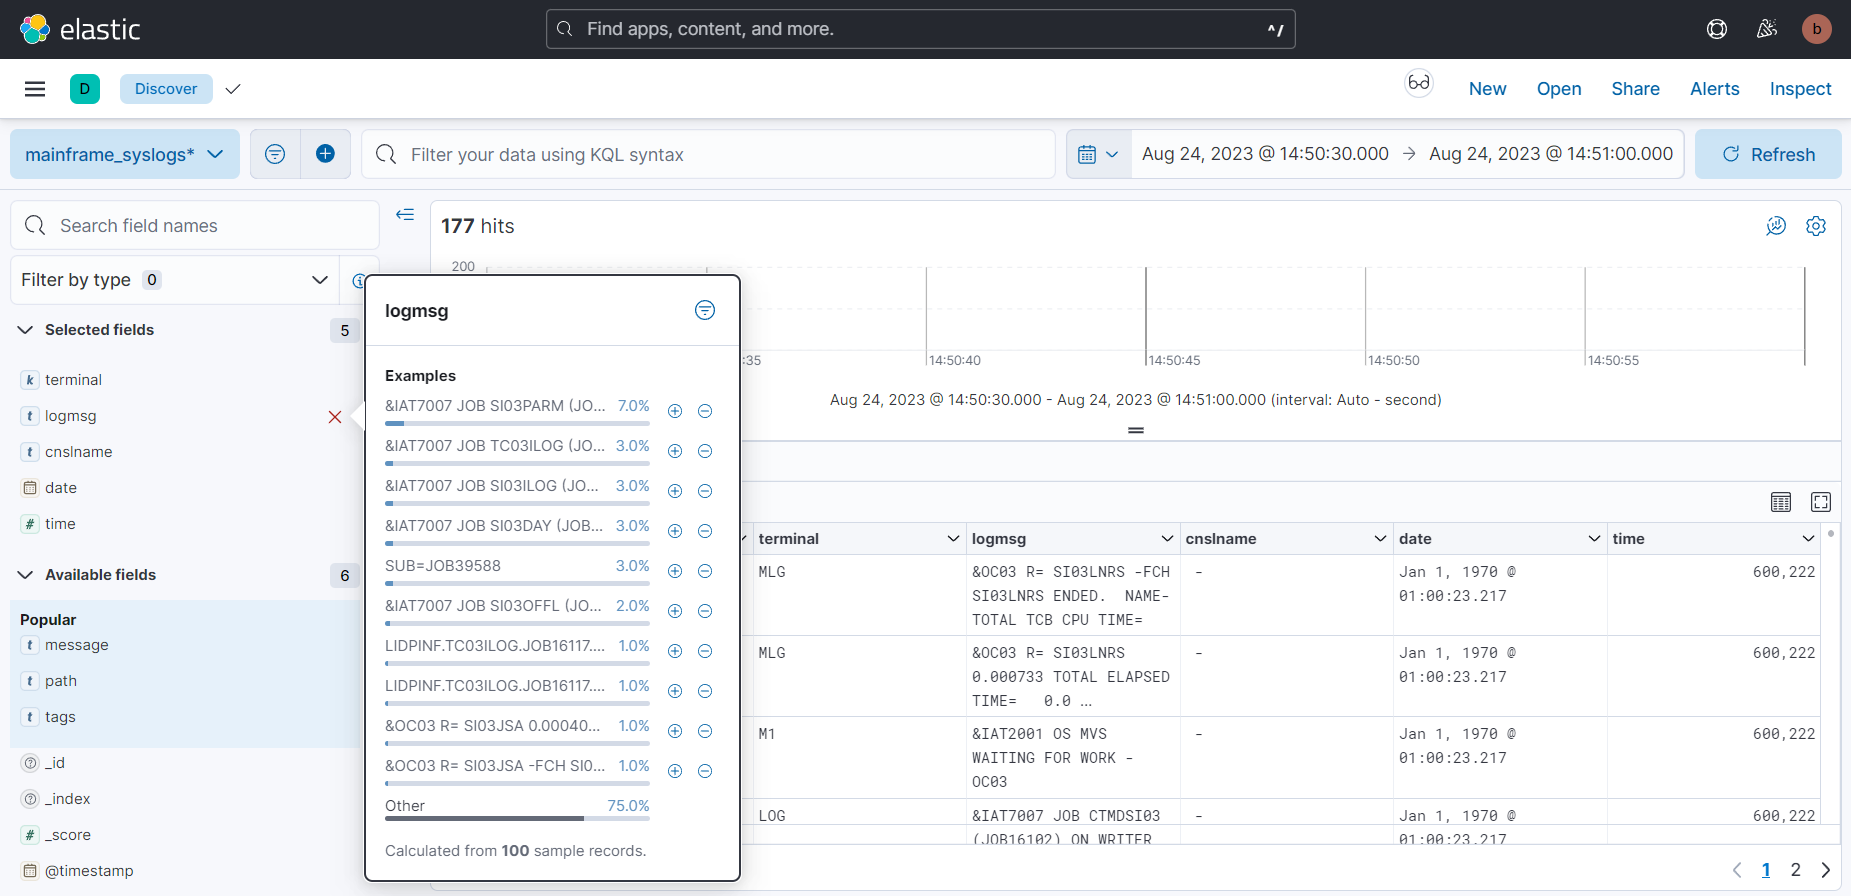
\includegraphics[width=0.50\linewidth]{bachproef//graphics/Kibana_stats_1.png}
    \caption{Statistieken 1}
    \label{fig:Statistieken 1}
\end{figure}

\begin{figure}[h]
    \centering
    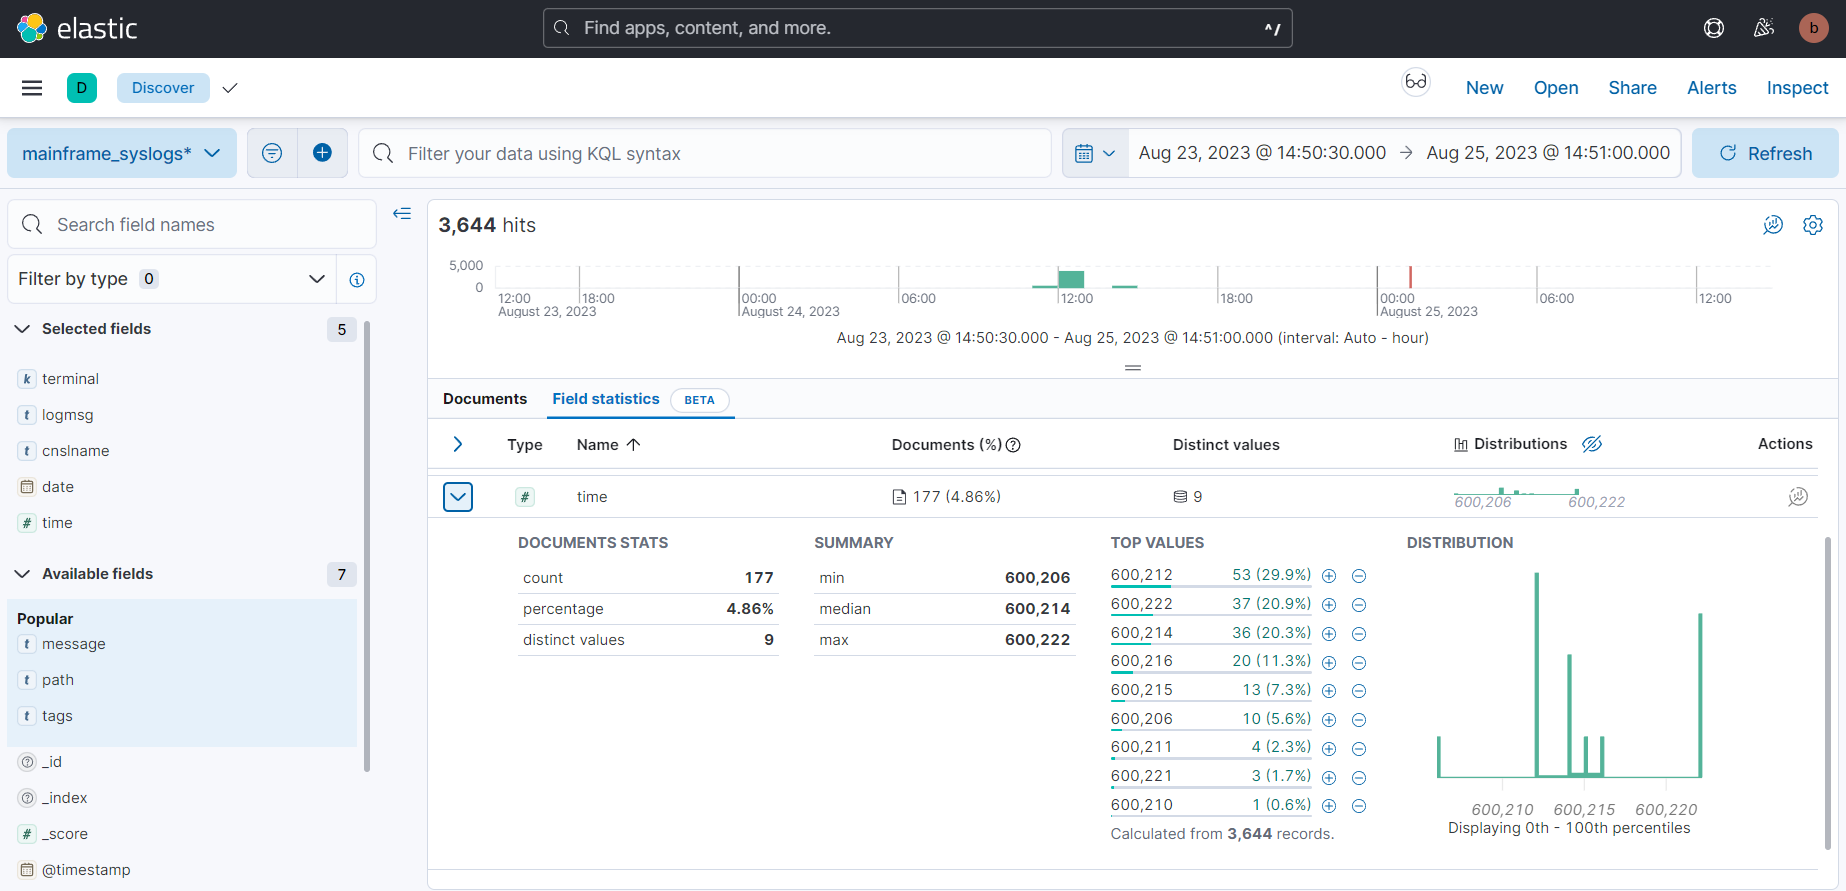
\includegraphics[width=0.50\linewidth]{Kibana_stats_2.png}
    \caption{Statistieken 2}
    \label{fig:Statistieken 2}
\end{figure}
\clearpage
\subsubsection{Paneel vier}
Dit paneel is bedoeld om het meest recente log te kunnen bekijken. Deze optie was al beschikbaar bij het openen van "Mainframe systemlogs." Alleen moesten de gewenste velden en datum worden geselecteerd. Bovendien kan dit eenvoudig worden gefilterd om relevante gegevens te bekijken.

\begin{figure}[h]
    \centering
    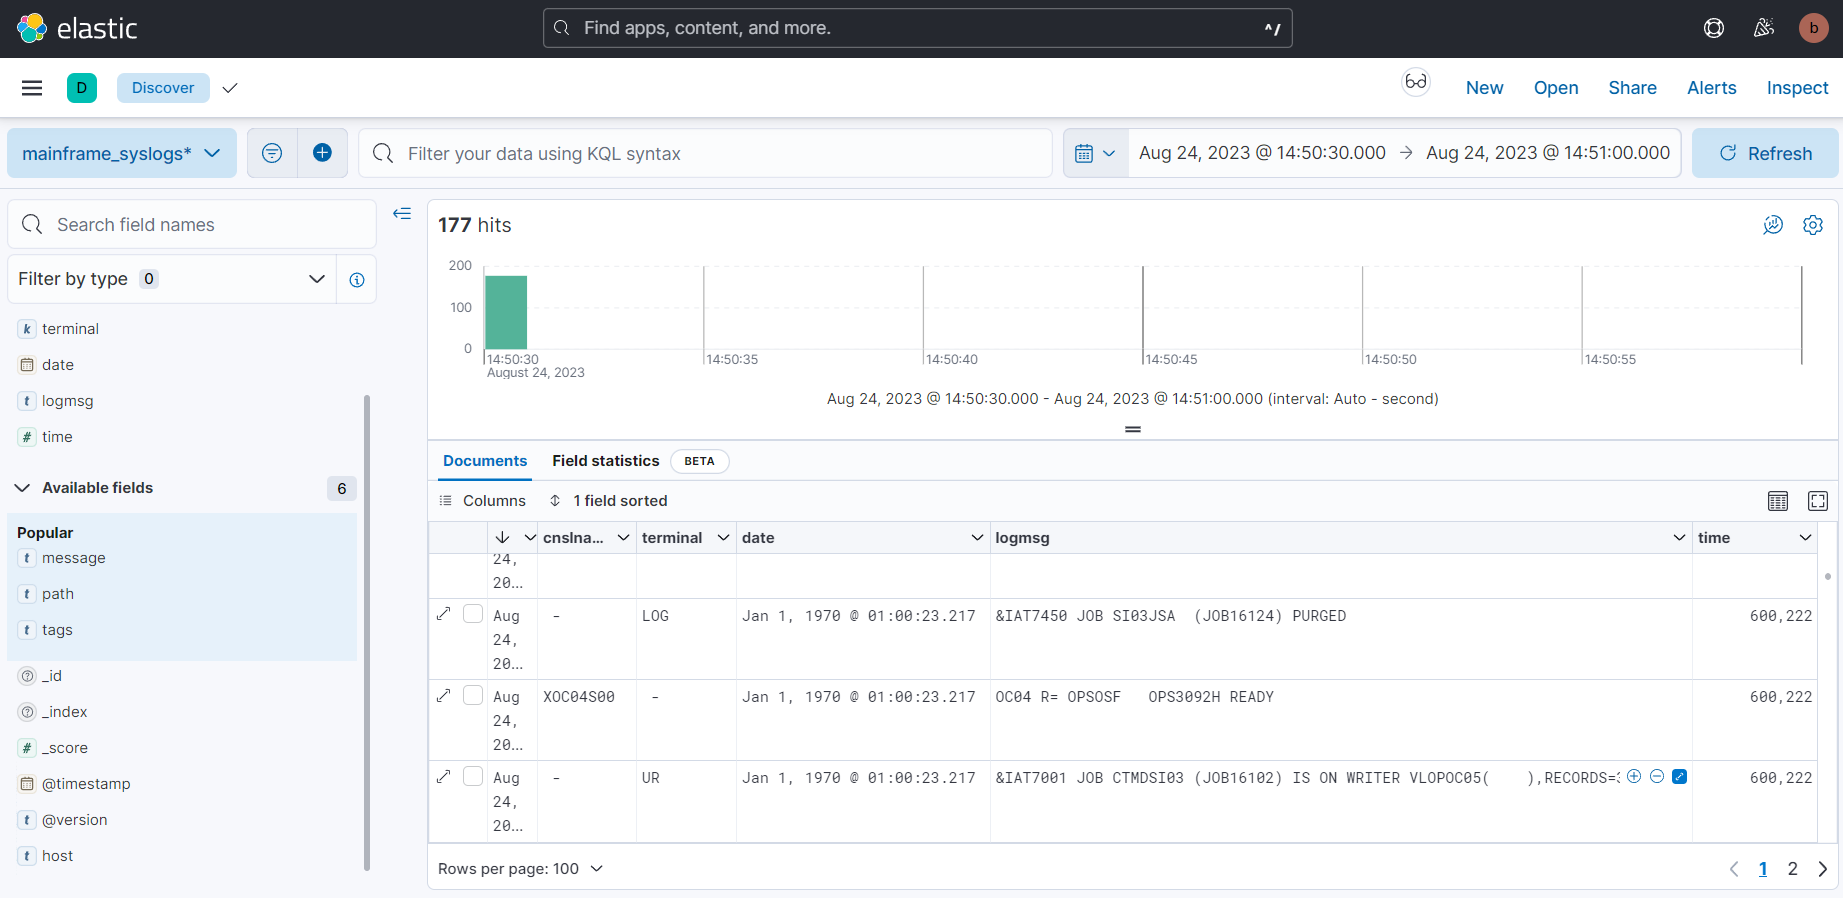
\includegraphics[width=0.50\linewidth]{Kibana_recent_log.png}
    \caption{De meest recente log}
    \label{fig:De meest recente log}
\end{figure}

\subsubsection{Paneel vijf}
Paneel 5 van de mockup is een basis tekstpaneel. Voor dit paneel is geen extra werk nodig.

\subsection{Kibana-dashboard}
Hoewel er geen dashboard is gemaakt, kan worden geconcludeerd uit de eerdere tests dat het mogelijk is om de mockup nauwkeurig te repliceren in Kibana. Hierdoor kan de mockup worden gebruikt als een nauwkeurige representatie voor de conclusies. Al deze panelen waren zeer eenvoudig te maken door op "create visualisation" te klikken, zoals weergegeven in de rechterbovenhoek van figuur 5.3. Daarna was het een kwestie van testen welke velden het beste werkten met welke visualisaties. Het is veilig om te concluderen dat het niet veel extra werk zou zijn geweest om deze visualisaties op te nemen in een dashboard.
